\documentclass{standalone}
\usepackage{tikz}
\usetikzlibrary{patterns, positioning}


\begin{document}
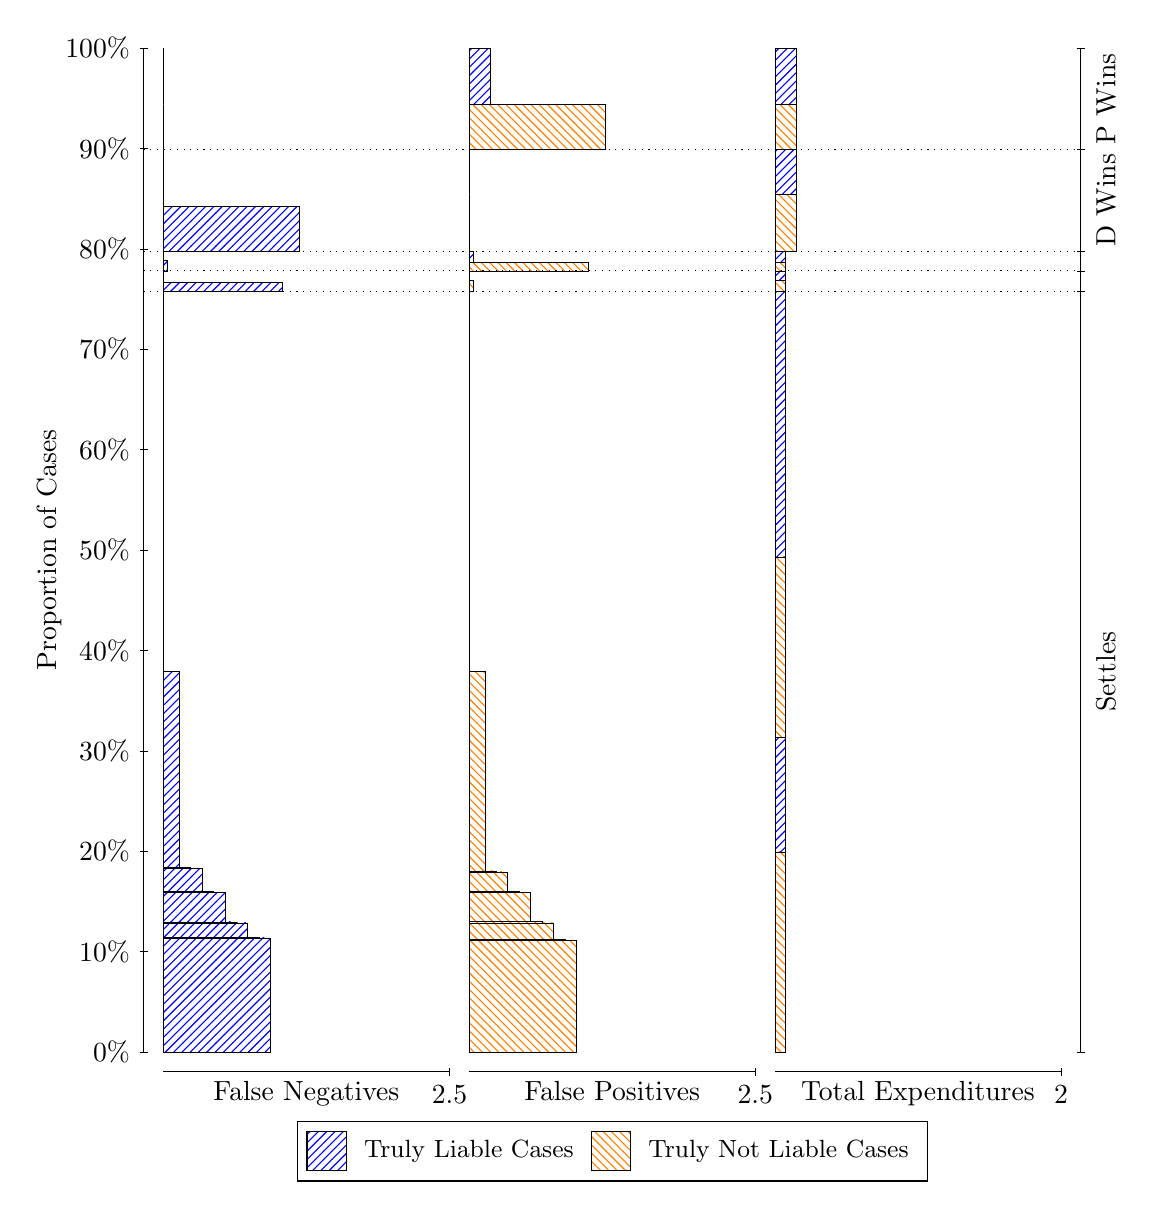
\begin{tikzpicture}
\draw[black, very thin] (1.5,1.75) -- (1.5,14.5);
\node[rotate=90, text=black, anchor=center] at (0.3, 8.125) {Proportion of Cases};
\draw[black, very thin] (1.45,1.75) -- (1.55,1.75);
\node[text=black, anchor=east] at (1.45, 1.75) {0\%};
\draw[black, very thin] (1.45,3.025) -- (1.55,3.025);
\node[text=black, anchor=east] at (1.45, 3.025) {10\%};
\draw[black, very thin] (1.45,4.3) -- (1.55,4.3);
\node[text=black, anchor=east] at (1.45, 4.3) {20\%};
\draw[black, very thin] (1.45,5.575) -- (1.55,5.575);
\node[text=black, anchor=east] at (1.45, 5.575) {30\%};
\draw[black, very thin] (1.45,6.85) -- (1.55,6.85);
\node[text=black, anchor=east] at (1.45, 6.85) {40\%};
\draw[black, very thin] (1.45,8.125) -- (1.55,8.125);
\node[text=black, anchor=east] at (1.45, 8.125) {50\%};
\draw[black, very thin] (1.45,9.4) -- (1.55,9.4);
\node[text=black, anchor=east] at (1.45, 9.4) {60\%};
\draw[black, very thin] (1.45,10.675) -- (1.55,10.675);
\node[text=black, anchor=east] at (1.45, 10.675) {70\%};
\draw[black, very thin] (1.45,11.95) -- (1.55,11.95);
\node[text=black, anchor=east] at (1.45, 11.95) {80\%};
\draw[black, very thin] (1.45,13.225) -- (1.55,13.225);
\node[text=black, anchor=east] at (1.45, 13.225) {90\%};
\draw[black, very thin] (1.45,14.5) -- (1.55,14.5);
\node[text=black, anchor=east] at (1.45, 14.5) {100\%};

\draw[black, very thin] (13.4,1.75) -- (13.4,14.5);
\draw[black, very thin] (13.35,1.75) -- (13.45,1.75);
\node[anchor=west] at (13.35, 1.75) {};
\draw[black, very thin] (13.35,11.41) -- (13.45,11.41);
\node[anchor=west] at (13.35, 11.41) {};
\draw[black, very thin] (13.35,11.669) -- (13.45,11.669);
\node[anchor=west] at (13.35, 11.669) {};
\draw[black, very thin] (13.35,11.921) -- (13.45,11.921);
\node[anchor=west] at (13.35, 11.921) {};
\draw[black, very thin] (13.35,13.21) -- (13.45,13.21);
\node[anchor=west] at (13.35, 13.21) {};
\draw[black, very thin] (13.35,14.5) -- (13.45,14.5);
\node[anchor=west] at (13.35, 14.5) {};

\draw[black, very thin, pattern color=blue, pattern=north east lines] (1.75,1.75) rectangle (3.1125,3.1982);
\draw[black, very thin, pattern color=blue, pattern=north east lines] (1.75,3.1982) rectangle (2.9672,3.2075);
\draw[black, very thin, pattern color=blue, pattern=north east lines] (1.75,3.2075) rectangle (2.8218,3.3903);
\draw[black, very thin, pattern color=blue, pattern=north east lines] (1.75,3.3903) rectangle (2.6765,3.4031);
\draw[black, very thin, pattern color=blue, pattern=north east lines] (1.75,3.4031) rectangle (2.5312,3.7738);
\draw[black, very thin, pattern color=blue, pattern=north east lines] (1.75,3.7738) rectangle (2.3858,3.7905);
\draw[black, very thin, pattern color=blue, pattern=north east lines] (1.75,3.7905) rectangle (2.2405,4.079);
\draw[black, very thin, pattern color=blue, pattern=north east lines] (1.75,4.079) rectangle (2.0952,4.0916);
\draw[black, very thin, pattern color=blue, pattern=north east lines] (1.75,4.0916) rectangle (1.9498,6.5798);
\draw[black, very thin, pattern color=orange, pattern=north west lines] (1.75,6.5798) rectangle (1.75,11.41);
\draw[black, very thin, pattern color=blue, pattern=north east lines] (1.75,11.41) rectangle (3.2578,11.526);
\draw[black, very thin, pattern color=orange, pattern=north west lines] (1.75,11.526) rectangle (1.75,11.669);
\draw[black, very thin, pattern color=blue, pattern=north east lines] (1.75,11.669) rectangle (1.8045,11.808);
\draw[black, very thin, pattern color=orange, pattern=north west lines] (1.75,11.808) rectangle (1.75,11.921);
\draw[black, very thin, pattern color=blue, pattern=north east lines] (1.75,11.921) rectangle (3.4758,12.491);
\draw[black, very thin, pattern color=orange, pattern=north west lines] (1.75,12.491) rectangle (1.75,13.21);
\draw[black, very thin, pattern color=orange, pattern=north west lines] (1.75,13.21) rectangle (1.75,13.781);
\draw[black, very thin, pattern color=blue, pattern=north east lines] (1.75,13.781) rectangle (1.75,14.5);
\draw[black, very thin, pattern color=orange, pattern=north west lines] (5.6333,1.75) rectangle (6.9958,3.1678);
\draw[black, very thin, pattern color=orange, pattern=north west lines] (5.6333,3.1678) rectangle (6.8505,3.1771);
\draw[black, very thin, pattern color=orange, pattern=north west lines] (5.6333,3.1771) rectangle (6.7052,3.3902);
\draw[black, very thin, pattern color=orange, pattern=north west lines] (5.6333,3.3902) rectangle (6.5598,3.4036);
\draw[black, very thin, pattern color=orange, pattern=north west lines] (5.6333,3.4036) rectangle (6.4145,3.7744);
\draw[black, very thin, pattern color=orange, pattern=north west lines] (5.6333,3.7744) rectangle (6.2692,3.7779);
\draw[black, very thin, pattern color=orange, pattern=north west lines] (5.6333,3.7779) rectangle (6.2692,3.7905);
\draw[black, very thin, pattern color=orange, pattern=north west lines] (5.6333,3.7905) rectangle (6.1238,4.0378);
\draw[black, very thin, pattern color=orange, pattern=north west lines] (5.6333,4.0378) rectangle (5.9785,4.0504);
\draw[black, very thin, pattern color=orange, pattern=north west lines] (5.6333,4.0504) rectangle (5.8332,6.5798);
\draw[black, very thin, pattern color=blue, pattern=north east lines] (5.6333,6.5798) rectangle (5.6333,11.41);
\draw[black, very thin, pattern color=orange, pattern=north west lines] (5.6333,11.41) rectangle (5.6878,11.553);
\draw[black, very thin, pattern color=blue, pattern=north east lines] (5.6333,11.553) rectangle (5.6333,11.669);
\draw[black, very thin, pattern color=orange, pattern=north west lines] (5.6333,11.669) rectangle (7.1412,11.781);
\draw[black, very thin, pattern color=blue, pattern=north east lines] (5.6333,11.781) rectangle (5.6878,11.921);
\draw[black, very thin, pattern color=orange, pattern=north west lines] (5.6333,11.921) rectangle (5.6333,12.64);
\draw[black, very thin, pattern color=blue, pattern=north east lines] (5.6333,12.64) rectangle (5.6333,13.21);
\draw[black, very thin, pattern color=orange, pattern=north west lines] (5.6333,13.21) rectangle (7.3592,13.781);
\draw[black, very thin, pattern color=blue, pattern=north east lines] (5.6333,13.781) rectangle (5.9058,14.5);
\draw[black, very thin, pattern color=orange, pattern=north west lines] (9.5167,1.75) rectangle (9.6529,4.292);
\draw[black, very thin, pattern color=blue, pattern=north east lines] (9.5167,4.292) rectangle (9.6529,5.7495);
\draw[black, very thin, pattern color=orange, pattern=north west lines] (9.5167,5.7495) rectangle (9.6529,8.0373);
\draw[black, very thin, pattern color=blue, pattern=north east lines] (9.5167,8.0373) rectangle (9.6529,11.41);
\draw[black, very thin, pattern color=orange, pattern=north west lines] (9.5167,11.41) rectangle (9.6529,11.553);
\draw[black, very thin, pattern color=blue, pattern=north east lines] (9.5167,11.553) rectangle (9.6529,11.669);
\draw[black, very thin, pattern color=orange, pattern=north west lines] (9.5167,11.669) rectangle (9.6529,11.781);
\draw[black, very thin, pattern color=blue, pattern=north east lines] (9.5167,11.781) rectangle (9.6529,11.921);
\draw[black, very thin, pattern color=orange, pattern=north west lines] (9.5167,11.921) rectangle (9.7892,12.64);
\draw[black, very thin, pattern color=blue, pattern=north east lines] (9.5167,12.64) rectangle (9.7892,13.21);
\draw[black, very thin, pattern color=orange, pattern=north west lines] (9.5167,13.21) rectangle (9.7892,13.781);
\draw[black, very thin, pattern color=blue, pattern=north east lines] (9.5167,13.781) rectangle (9.7892,14.5);
\draw[black, dotted] (1.5,11.41) -- (13.4,11.41);
\draw[black, dotted] (1.5,11.669) -- (13.4,11.669);
\draw[black, dotted] (1.5,11.921) -- (13.4,11.921);
\draw[black, dotted] (1.5,13.21) -- (13.4,13.21);
\draw[black, very thin] (1.75,1.5) -- (5.3833,1.5);
\node[text=black, anchor=north] at (3.5667, 1.5) {False Negatives};
\draw[black, very thin] (5.3833,1.45) -- (5.3833,1.55);
\node[text=black, anchor=north] at (5.3833, 1.45) {2.5};

\draw[black, very thin] (5.6333,1.5) -- (9.2667,1.5);
\node[text=black, anchor=north] at (7.45, 1.5) {False Positives};
\draw[black, very thin] (9.2667,1.45) -- (9.2667,1.55);
\node[text=black, anchor=north] at (9.2667, 1.45) {2.5};

\draw[black, very thin] (9.5167,1.5) -- (13.15,1.5);
\node[text=black, anchor=north] at (11.333, 1.5) {Total Expenditures};
\draw[black, very thin] (13.15,1.45) -- (13.15,1.55);
\node[text=black, anchor=north] at (13.15, 1.45) {2};

\node[text=black, centered, rotate=90] at (13.72, 6.5798) {Settles};


\node[text=black, centered, rotate=90] at (13.72, 12.565) {D Wins};
\node[text=black, centered, rotate=90] at (13.72, 13.855) {P Wins};

\draw (7.449999999999999,1.5) node[draw=none] (baseCoordinate) {};
\begin{scope}[align=center]
        \matrix[scale=0.5, draw=black, below=0.5cm of baseCoordinate, nodes={draw}, column sep=0.1cm]{
            \node[rectangle, draw, minimum width=0.5cm, minimum height=0.5cm, pattern color=blue, pattern=north east lines] {}; &
            \node[draw=none, font=\small, text=black] (B) {Truly Liable Cases}; &
            \node[rectangle, draw, minimum width=0.5cm, minimum height=0.5cm, pattern color=orange, pattern=north west lines] {}; &
            \node[draw=none, font=\small, text=black] (B) {Truly Not Liable Cases}; \\
            };
\end{scope}

\end{tikzpicture}
\end{document}